\begin{tabularx}{\textwidth}{Y}
  {\large University of Evansville Lesson Plan Format 8/29/2025} \\
  \arrayrulecolor{blue} \hline \\
\end{tabularx}


\arrayrulecolor{black} 
\begin{tabularx}{\textwidth}{|X|X|}
  \hline 
  \textcolor{blue}{Name:} Randall Helzerman         &   \textcolor{blue}{Student ID Number:} 0128861 \\
  \hline 
  \textcolor{blue}{Course Number:} EDUC-497-03 2025FA &   \textcolor{blue}{Instructor Name:} Dr. Laura Watkins\\
  \hline 
\end{tabularx}
\arrayrulecolor{black}

\vskip 10pt

\begin{tabularx}{\textwidth}{Y}
  {\bf Lesson Overview} \\
\end{tabularx}
\arrayrulecolor{black}


\arrayrulecolor{black} 
\begin{tabularx}{\textwidth}{|X|X|}
  \hline 
  \textbf{Lesson Title:} \\
  
  \hline 
  \textbf{Subject:} Math\\
  
  \hline 
      {
        \begin{tabularx}{\textwidth}{X|X}
          \hskip -6pt
          \textbf{Duration of Lesson:} & \textbf{Grade Level(s)/Course:} 8th grade\\
        \end{tabularx}
      } \\
      
      \hline
      
      \textbf{Lesson Description: {\tiny (Describe the primary nature e.g. hands-on, direct instruction, inquiry, project based etc. of the lesson)}} \\
      
      \hline
      
      \textbf{Standards and/or Indicator(s):} {\tiny Cut and paste
        from IDOE website here. Feel free to replicate the
        descriptors listed below to include more standards in this
        section.} \\
      
      \textbf{Indiana Standard number:} \\
      \textbf{Text:} \\
      \hline
      
      \textbf{Learning Objective(s)/Target:} {\tiny What do I want students to learn and be able to do at the end of the lesson? (I can statements)}
             {\begin{enumerate}
               \item Lorum
               \item ipsum
             \end{enumerate}} \\
             \hline
             
             \textbf{Lesson Resources/Technology: } {\tiny (What
               technology will I use? What technology will students
               use for this lesson? What resources will you and/or
               the students need for the lesson – books, mentor
               texts, etc.)} \\
             \hline
             
             \textbf{Key Vocabulary:} {\tiny List all key vocabulary words that will be taught to help students understand the concepts in the lesson.} \\
             \hline
\end{tabularx}
\arrayrulecolor{black}

\pagebreak

\begin{tabularx}{\textwidth}{|p{0.5in}|X|}
  \hline
  \centerline{\textbf{\large Time}} &  \textbf{\large Instructional Sequence } \\
  \hline
  \textbf{5 min} &  \textbf{\em Introduction/Anticipatory Set:}  \\

  & Draw the following figures on the promethean board: \\
  
  & 
  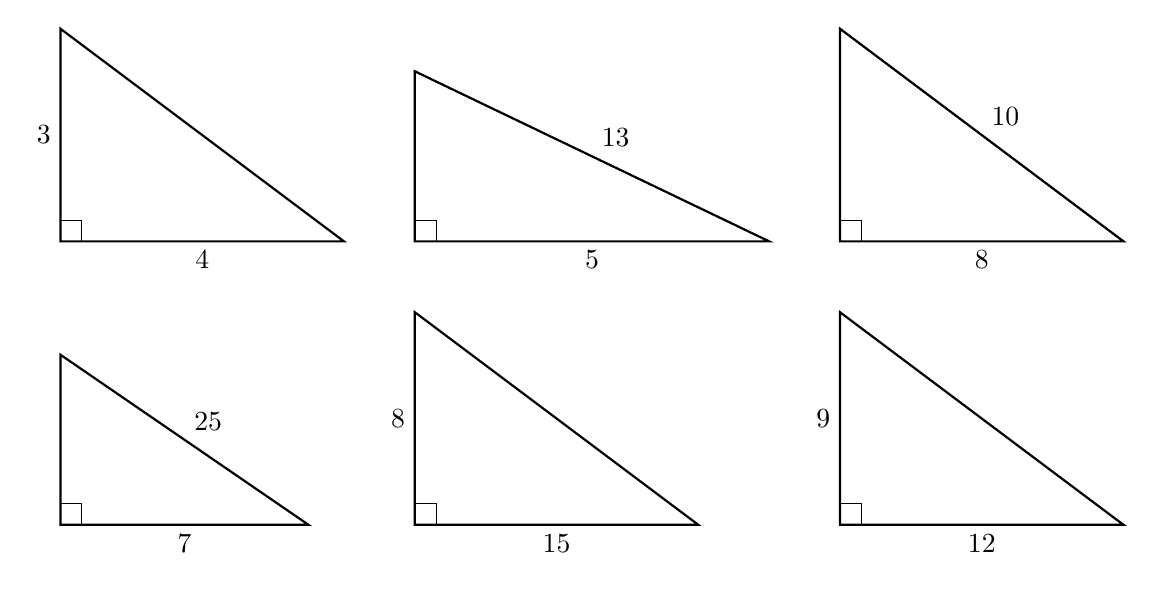
\begin{tikzpicture}[scale=0.9]
    
    % Row 1, Column 1 - Problem 1 (3-4-5 triangle)
    \begin{scope}[shift={(0,0)}]
      \draw[thick] (0,0) -- (4,0) -- (0,3) -- cycle;
      \draw (0.3,0) -- (0.3,0.3) -- (0,0.3);
      \node[below] at (2,0) {4};
      \node[left] at (0,1.5) {3};
    \end{scope}
    
    % Row 1, Column 2 - Problem 2 (5-12-13 triangle)
    \begin{scope}[shift={(5,0)}]
      \draw[thick] (0,0) -- (5,0) -- (0,2.4) -- cycle;
      \draw (0.3,0) -- (0.3,0.3) -- (0,0.3);
      \node[below] at (2.5,0) {5};
      \node[above right] at (2.5,1.2) {13};
    \end{scope}
    
    % Row 1, Column 3 - Problem 3 (6-8-10 triangle)
    \begin{scope}[shift={(11,0)}]
      \draw[thick] (0,0) -- (4,0) -- (0,3) -- cycle;
      \draw (0.3,0) -- (0.3,0.3) -- (0,0.3);
      \node[below] at (2,0) {8};
      \node[above right] at (2,1.5) {10};
    \end{scope}
    
    % Row 2, Column 1 - Problem 4 (7-24-25 triangle)
    \begin{scope}[shift={(0,-4)}]
      \draw[thick] (0,0) -- (3.5,0) -- (0,2.4) -- cycle;
      \draw (0.3,0) -- (0.3,0.3) -- (0,0.3);
      \node[below] at (1.75,0) {7};
      \node[above right] at (1.75,1.2) {25};
    \end{scope}
    
    % Row 2, Column 2 - Problem 5 (8-15-17 triangle)
    \begin{scope}[shift={(5,-4)}]
      \draw[thick] (0,0) -- (4,0) -- (0,3) -- cycle;
      \draw (0.3,0) -- (0.3,0.3) -- (0,0.3);
      \node[below] at (2,0) {15};
      \node[left] at (0,1.5) {8};
    \end{scope}
    
    % Row 2, Column 3 - Problem 6 (9-12-15 triangle)
    \begin{scope}[shift={(11,-4)}]
      \draw[thick] (0,0) -- (4,0) -- (0,3) -- cycle;
      \draw (0.3,0) -- (0.3,0.3) -- (0,0.3);
      \node[below] at (2,0) {12};
      \node[left] at (0,1.5) {9};
    \end{scope}
    
  \end{tikzpicture}  \\

  & Ask the students to write on their whiteboards what the labeled
  sides are for each triangle: Is it the hypoteneus, or a leg? \\
  
  \hline
  
  \textbf{} &

  \textbf{\em Demonstrate, Build, Apply Knowledge} {\tiny What
    meaningful activity will engate students, activate prior
    knowledge, and prepare students for learning objectives} \\
  
  \hline
  
  \textbf{} & \textbf{\em Depth of Knowledge Questions:} {\tiny
    Essential questions to extend higher level thinking) } \\

  \hline
  
  \textbf{} & \textbf{\em Guided Practice:} {\tiny (Check for
    understanding prior to independent work; “We do”)} \\
  
  \hline

  \textbf{} & \textbf{\em Independent Practice:} {\tiny (Individual
    practice, learning centers, reading, composing writing; “You do”)}
  \\
  
  \hline

  \textbf{} & \textbf{\em Assessment:} {\tiny (Evaluate level of
    student understanding. How will I know if students have achieved
    today’s learning target?)} \\
  \hline
  
  \textbf{} & \textbf{\em Wrap Up/Closing Activity/Reflection:} {\tiny
    (How will I reinforce/revisit the learning objective? Opportunity
    for formative assessment. Students reflect on evidence of learning
    – writing, reading, math target. How will we build on this
    learning?)} \\
  
  \hline
\end{tabularx}
  
\vskip 6pt

\begin{small}
\begin{tabularx}{\linewidth}{|p{2.1in}|X|}
  \hline
  \textbf{Differentiation/Accommodations and/or Modifications: } & \\
  \hline
  \textbf{Culturally Responsive Teaching/ Diversity and Inclusion: } & \\
  \hline
\end{tabularx}

\vskip 6pt

\begin{tabularx}{\linewidth}{|X|}
  \hline
  \textbf{Self-Reflection:} \\
  \textbf{My Teaching:} 
  \begin{enumerate}
  \item .
  \item .
  \end{enumerate} \\
  
  \textbf{The Students:}
  \begin{enumerate}
  \item .
  \item .
  \end{enumerate} \\
  
  \textbf{The Lesson:}
  \begin{enumerate}
  \item .
  \item .
  \end{enumerate} \\
  
  \hline
\end{tabularx}
\end{small}
